\documentclass[a4paper, 14pt]{extarticle}

% Поля
%--------------------------------------
\usepackage{geometry}
\geometry{a4paper,tmargin=2cm,bmargin=2cm,lmargin=3cm,rmargin=1cm}
%--------------------------------------


%Russian-specific packages
%--------------------------------------
\usepackage[T2A]{fontenc}
\usepackage[utf8]{inputenc}
\usepackage[english, main=russian]{babel}
%--------------------------------------

\usepackage{textcomp}

% Красная строка
%--------------------------------------
\usepackage{indentfirst}
%--------------------------------------


%Graphics
%--------------------------------------
\usepackage{graphicx}
\graphicspath{ {./images/} }
\usepackage{wrapfig}
%--------------------------------------

% Полуторный интервал
%--------------------------------------
\linespread{1.3}
%--------------------------------------

%Выравнивание и переносы
%--------------------------------------
% Избавляемся от переполнений
\sloppy
% Запрещаем разрыв страницы после первой строки абзаца
\clubpenalty=10000
% Запрещаем разрыв страницы после последней строки абзаца
\widowpenalty=10000
%--------------------------------------

%Списки
\usepackage{enumitem}

%Подписи
\usepackage{caption}

%Гиперссылки
\usepackage{hyperref}

\hypersetup {
	unicode=true
}

%Рисунки
%--------------------------------------
\DeclareCaptionLabelSeparator*{emdash}{~--- }
\captionsetup[figure]{labelsep=emdash,font=onehalfspacing,position=bottom}
%--------------------------------------

\usepackage{tempora}

%Листинги
%--------------------------------------
\usepackage{listings}
\lstset{
  basicstyle=\ttfamily\footnotesize,
  %basicstyle=\footnotesize\AnkaCoder,        % the size of the fonts that are used for the code
  breakatwhitespace=false,         % sets if automatic breaks shoulbd only happen at whitespace
  breaklines=true,                 % sets automatic line breaking
  captionpos=t,                    % sets the caption-position to bottom
  inputencoding=utf8,
  frame=single,                    % adds a frame around the code
  keepspaces=true,                 % keeps spaces in text, useful for keeping indentation of code (possibly needs columns=flexible)
  keywordstyle=\bf,       % keyword style
  numbers=left,                    % where to put the line-numbers; possible values are (none, left, right)
  numbersep=5pt,                   % how far the line-numbers are from the code
  xleftmargin=25pt,
  xrightmargin=25pt,
  showspaces=false,                % show spaces everywhere adding particular underscores; it overrides 'showstringspaces'
  showstringspaces=false,          % underline spaces within strings only
  showtabs=false,                  % show tabs within strings adding particular underscores
  stepnumber=1,                    % the step between two line-numbers. If it's 1, each line will be numbered
  tabsize=2,                       % sets default tabsize to 8 spaces
  title=\lstname                   % show the filename of files included with \lstinputlisting; also try caption instead of title
}
%--------------------------------------

%%% Математические пакеты %%%
%--------------------------------------
\usepackage{amsthm,amsfonts,amsmath,amssymb,amscd}  % Математические дополнения от AMS
\usepackage{mathtools}                              % Добавляет окружение multlined
\usepackage[perpage]{footmisc}
%--------------------------------------

%--------------------------------------
%			НАЧАЛО ДОКУМЕНТА
%--------------------------------------

\begin{document}

%--------------------------------------
%			ТИТУЛЬНЫЙ ЛИСТ
%--------------------------------------
\begin{titlepage}
\thispagestyle{empty}
\newpage


%Шапка титульного листа
%--------------------------------------
\vspace*{-60pt}
\hspace{-65pt}
\begin{minipage}{0.3\textwidth}
\hspace*{-20pt}\centering

\includegraphics[width=\textwidth]{emblem}
\end{minipage}
\begin{minipage}{0.67\textwidth}\small \textbf{
\vspace*{-0.7ex}
\hspace*{-6pt}\centerline{Министерство науки и высшего образования Российской Федерации}
\vspace*{-0.7ex}
\centerline{Федеральное государственное бюджетное образовательное учреждение }
\vspace*{-0.7ex}
\centerline{высшего образования}
\vspace*{-0.7ex}
\centerline{<<Московский государственный технический университет}
\vspace*{-0.7ex}
\centerline{имени Н.Э. Баумана}
\vspace*{-0.7ex}
\centerline{(национальный исследовательский университет)>>}
\vspace*{-0.7ex}
\centerline{(МГТУ им. Н.Э. Баумана)}}
\end{minipage}
%--------------------------------------

%Полосы
%--------------------------------------
\vspace{-25pt}
\hspace{-35pt}\rule{\textwidth}{2.3pt}

\vspace*{-20.3pt}
\hspace{-35pt}\rule{\textwidth}{0.4pt}
%--------------------------------------

\vspace{1.5ex}
\hspace{-35pt} \noindent \small ФАКУЛЬТЕТ\hspace{80pt} <<Информатика и системы управления>>

\vspace*{-16pt}
\hspace{47pt}\rule{0.83\textwidth}{0.4pt}

\vspace{0.5ex}
\hspace{-35pt} \noindent \small КАФЕДРА\hspace{50pt} <<Теоретическая информатика и компьютерные технологии>>

\vspace*{-16pt}
\hspace{30pt}\rule{0.866\textwidth}{0.4pt}

\vspace{11em}

\begin{center}
\Large {\bf Рубежный контроль № 3} \\
\large {\bf по курсу <<Разработка мобильных приложений>>} \\
\large <<Взаимодействие приложения на Kotlin с Firebase>>
\end{center}\normalsize

\vspace{8em}


\begin{flushright}
  {Студентка группы ИУ9-72Б Самохвалова П. С. \hspace*{15pt}\\
  \vspace{2ex}
  Преподаватель Посевин Д. П.\hspace*{15pt}}
\end{flushright}

\bigskip

\vfill


\begin{center}
\textsl{Москва 2023}
\end{center}
\end{titlepage}
%--------------------------------------
%		КОНЕЦ ТИТУЛЬНОГО ЛИСТА
%--------------------------------------

\renewcommand{\ttdefault}{pcr}

\setlength{\tabcolsep}{3pt}
\newpage
\setcounter{page}{2}

\section{Задание}\label{Sect::task}

Реализовать мобильное приложение с матрицей 3x3 с возможностью ввода значений и сохранением значений в Firebase.

\section{Практическая реализация}\label{Sect::code}

Исходный код программы представлен в листинге~\ref{lst:code1}.

\begin{lstlisting}[language={},caption={},label={lst:code1}]
package com.example.kotlin_auth5_klicker_fb

import android.content.Intent
import androidx.appcompat.app.AppCompatActivity
import android.os.Bundle
import android.view.View
import android.widget.Button
import android.widget.Toast
import com.google.android.gms.tasks.OnCompleteListener
import com.google.firebase.auth.AuthResult
import com.google.firebase.auth.FirebaseAuth
import com.google.firebase.database.DatabaseReference
import com.google.firebase.database.FirebaseDatabase
import android.widget.EditText
import androidx.core.widget.addTextChangedListener


class MainActivity : AppCompatActivity() {
    private lateinit var editText_00: EditText
    private lateinit var editText_01: EditText
    private lateinit var editText_02: EditText
    private lateinit var editText_10: EditText
    private lateinit var editText_11: EditText
    private lateinit var editText_12: EditText
    private lateinit var editText_20: EditText
    private lateinit var editText_21: EditText
    private lateinit var editText_22: EditText
    private val database = FirebaseDatabase.getInstance("https://mobile-5276e-default-rtdb.asia-southeast1.firebasedatabase.app/").reference
    private val Text_00 = database.child("a00")
    private val Text_01 = database.child("a01")
    private val Text_02 = database.child("a02")
    private val Text_10 = database.child("a10")
    private val Text_11 = database.child("a11")
    private val Text_12 = database.child("a12")
    private val Text_20 = database.child("a20")
    private val Text_21 = database.child("a21")
    private val Text_22 = database.child("a22")

    override fun onCreate(savedInstanceState: Bundle?) {
        super.onCreate(savedInstanceState)
        setContentView(R.layout.activity_main)

        editText_00 = findViewById(R.id.editText_00)
        editText_01 = findViewById(R.id.editText_01)
        editText_02 = findViewById(R.id.editText_02)
        editText_10 = findViewById(R.id.editText_10)
        editText_11 = findViewById(R.id.editText_11)
        editText_12 = findViewById(R.id.editText_12)
        editText_20 = findViewById(R.id.editText_20)
        editText_21 = findViewById(R.id.editText_21)
        editText_22 = findViewById(R.id.editText_22)


        editText_00.addTextChangedListener { text ->
            Text_00.setValue(text.toString())
        }

        editText_01.addTextChangedListener { text ->
            Text_01.setValue(text.toString())
        }

        editText_02.addTextChangedListener { text ->
            Text_02.setValue(text.toString())
        }

        editText_10.addTextChangedListener { text ->
            Text_10.setValue(text.toString())
        }

        editText_11.addTextChangedListener { text ->
            Text_11.setValue(text.toString())
        }

        editText_12.addTextChangedListener { text ->
            Text_12.setValue(text.toString())
        }

        editText_20.addTextChangedListener { text ->
            Text_20.setValue(text.toString())
        }

        editText_21.addTextChangedListener { text ->
            Text_21.setValue(text.toString())
        }

        editText_22.addTextChangedListener { text ->
            Text_22.setValue(text.toString())
        }
    }
}


<?xml version="1.0" encoding="utf-8"?>
<LinearLayout xmlns:android="http://schemas.android.com/apk/res/android"
    android:layout_width="match_parent"
    android:layout_height="match_parent"
    android:orientation="vertical">

    <LinearLayout
        android:layout_width="wrap_content"
        android:layout_height="wrap_content"
        android:orientation="horizontal">

        <EditText
            android:id="@+id/editText_00"
            android:layout_width="wrap_content"
            android:layout_height="wrap_content"
            android:inputType="number"
            android:ems="5" />

        <EditText
            android:id="@+id/editText_01"
            android:layout_width="wrap_content"
            android:layout_height="wrap_content"
            android:inputType="number"
            android:ems="5" />

        <EditText
            android:id="@+id/editText_02"
            android:layout_width="wrap_content"
            android:layout_height="wrap_content"
            android:inputType="number"
            android:ems="5" />

    </LinearLayout>

    <LinearLayout
        android:layout_width="wrap_content"
        android:layout_height="wrap_content"
        android:orientation="horizontal">

        <EditText
            android:id="@+id/editText_10"
            android:layout_width="wrap_content"
            android:layout_height="wrap_content"
            android:inputType="number"
            android:ems="5" />

        <EditText
            android:id="@+id/editText_11"
            android:layout_width="wrap_content"
            android:layout_height="wrap_content"
            android:inputType="number"
            android:ems="5" />

        <EditText
            android:id="@+id/editText_12"
            android:layout_width="wrap_content"
            android:layout_height="wrap_content"
            android:inputType="number"
            android:ems="5" />

    </LinearLayout>

    <LinearLayout
        android:layout_width="wrap_content"
        android:layout_height="wrap_content"
        android:orientation="horizontal">

        <EditText
            android:id="@+id/editText_20"
            android:layout_width="wrap_content"
            android:layout_height="wrap_content"
            android:inputType="number"
            android:ems="5" />

        <EditText
            android:id="@+id/editText_21"
            android:layout_width="wrap_content"
            android:layout_height="wrap_content"
            android:inputType="number"
            android:ems="5" />

        <EditText
            android:id="@+id/editText_22"
            android:layout_width="wrap_content"
            android:layout_height="wrap_content"
            android:inputType="number"
            android:ems="5" />

    </LinearLayout>

</LinearLayout>

\end{lstlisting}

\section{Результаты}\label{Sect::res}

Результаты работы программы представлены на рисунках~\ref{fig:img1}~--~\ref{fig:img5}.     

\begin{figure}[!htb]
	\centering
	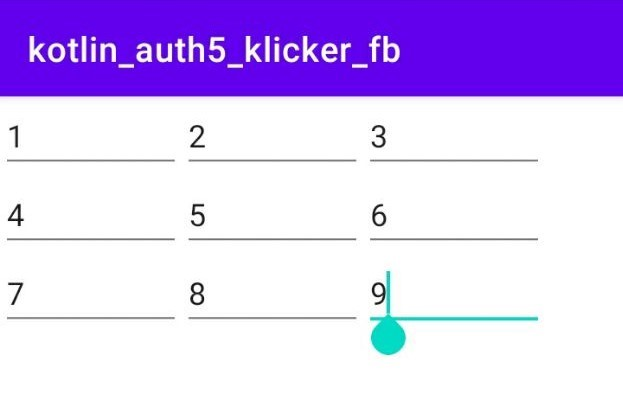
\includegraphics[width=0.8\textwidth]{img1}
\caption{Результаты}
\label{fig:img1}
\end{figure}

\begin{figure}[!htb]
	\centering
	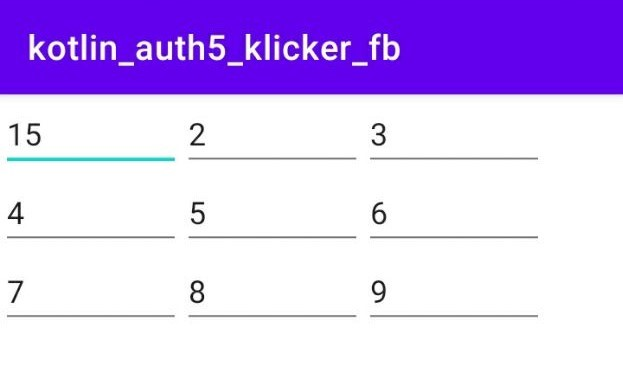
\includegraphics[width=0.8\textwidth]{img2}
\caption{Результаты}
\label{fig:img2}
\end{figure}

\begin{figure}[!htb]
	\centering
	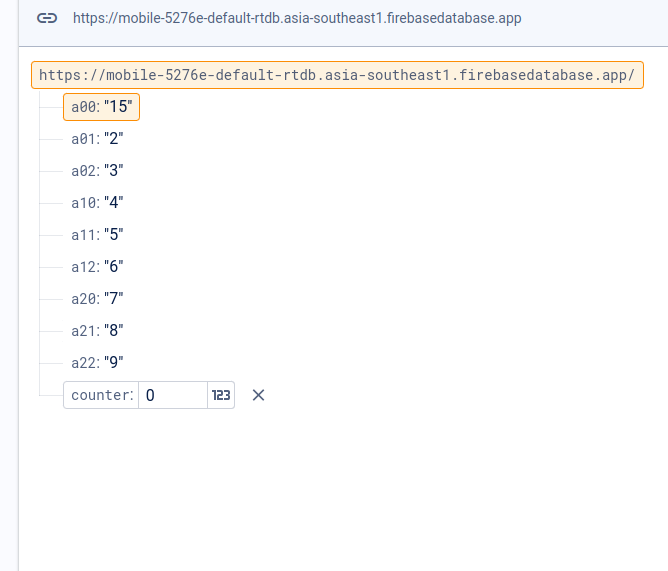
\includegraphics[width=0.8\textwidth]{img3}
\caption{Результаты}
\label{fig:img3}
\end{figure}

\begin{figure}[!htb]
	\centering
	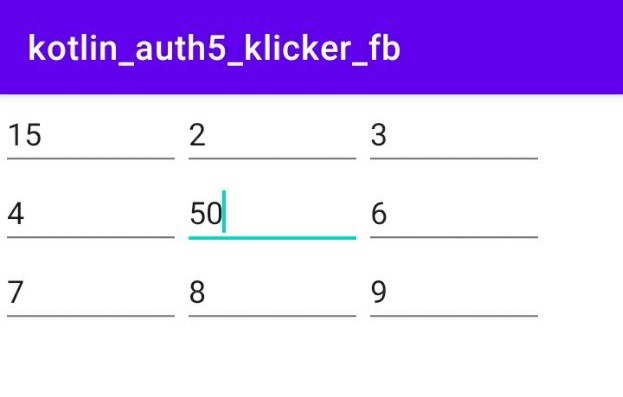
\includegraphics[width=0.8\textwidth]{img4}
\caption{Результаты}
\label{fig:img4}
\end{figure}

\begin{figure}[!htb]
	\centering
	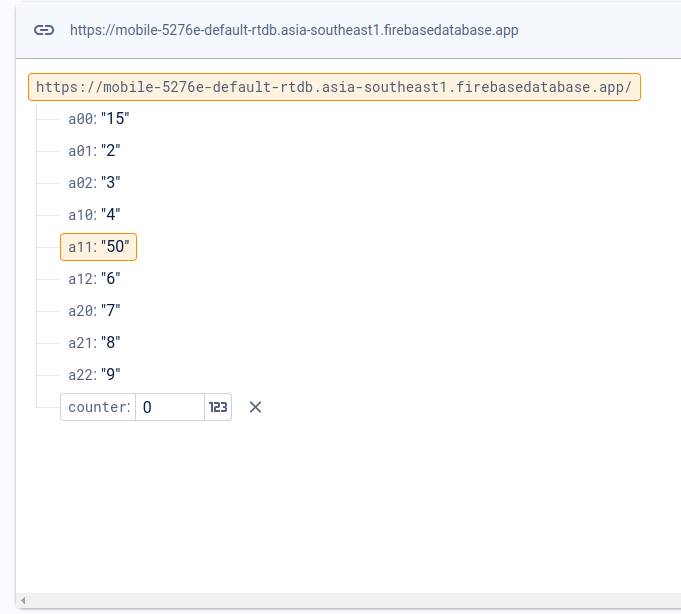
\includegraphics[width=0.8\textwidth]{img5}
\caption{Результаты}
\label{fig:img5}
\end{figure}

\section{Выводы}\label{Sect::conclusion}

В результате выполнения рубежного контроля было реализовано мобильное приложение с матрицей 3x3 с возможностью ввода значений и сохранением значений в Firebase.

\end{document}
